\documentclass{journal}
\usepackage{graphics,graphicx}
\usepackage{hyperref}
\usepackage{fullpage}
\usepackage{pdflscape}
\usepackage{tikz}
\usepackage{gantt}
\usepackage{setspace}

\onehalfspacing

\begin{document}
\bibliographystyle{IEEE}
\title{Interactive Graduate Student Information Database}
\subtitle{Technical Proposal} 
\author{Kartik Thakore (250313003)\\kthakore@uwo.ca \and Parth Champaneri (250367669)\\pchampan@uwo.ca}
\maketitle

\begin{abstract}
We began the search for our fourth year project during our internship. Dr. Ladak visited us for our internship reviews alongside which, we had several discussions on possible final year projects. During our term at CIBC, we have gained first-hand experience of manual inefficient processes and have played a critical role in revamping several inefficient business processes by implementing automated workflow tools. When Dr. Ladak presented a problem with managing graduate students’ information at various faculties across the university, we knew our past expertise could be utilized to engineer an efficient solution for the university. Furthermore, as a past graduate chair of the faculty of Medical BioPhysics, Dr. Ladak's experience and feedback would be crucial to the success of this project. To acquire a better understanding of the problem, we had meetings with Ms. Wendy Hough, the Graduate Affairs Assistant in the Medical BioPhysics Program. While working to define the problem, we have gained an appreciation of the complexity and difficulty in managing graduate student data. In our proposal below we describe the problem, and our objectives during this project. We will also cover the scope of project management aspects in regards to the Agile methodology, project resource and strategic planning. Overall we are excited and enthusiastic about this initiative and its potential benefits for other graduate faculties in the future.
\end{abstract}

\section{Background}

The enrolment of Ontario graduate students is expected double by 2013, since 2005 \cite{con_high}.  One of the key issues is to administer and govern students' program milestones. Furthermore, a manual reporting mechanism is currently used where several reports are generated from the database of various students.
The current system is a large excel sheet and several cabinets of paper copies. The end-user has an increasingly difficult time in effectively managing 
the data. In addition the user needs to manually calculate critical dates to prompt graduate students for feedback. Therefore, the existing system is no longer scalable to the demands and the complexity of milestones and critical dates for the program. 

In our understanding of the problem, we would like to explore the concept of treating each student as a task which requires various rules and milestones. Application of the rules and milestones would conceptually define a process. Techniques of process engineering and management 
have been applied to student monitoring and tracking. Similar projects in the past have been met with some success and challenges \cite{flex}. 
Moreover an electronic system to manage administration can reduce burdens on students \cite{adv}. Prior solutions will help us avoid problems and follow best practices. 
Electronic systems to track and store data is a mature technology, and can be successfully applied to this problem. 

\section{Objectives}

To design and implement an Interactive Student Information Management System (SIMS) database for Graduate students that can track important dates from inception 
to completion of the program life cycle and help manage information on an efficient basis. Upon completion, this system will be used to manage graduate students 
in various faculties and provide effective reporting techniques, which will aid in tracking, resource and strategic planning.
\subsection{ Goals }
 Features of the program include:
\begin{itemize}
 \item{Track various milestones throughout the program including, but not limited to:}
 \begin{itemize}
   \item{ Name and Demographic information }
   \item{ Program Start-End Dates }
   \item{ Recording other information (Names of advisory committee members, outcome of an advisory committee meeting etc.) }
  \end{itemize}
  \item{ E-mail reminders (Standard text for that milestone and a way of sending that reminder via e-mail) }
  \item{ RFID and e-applications will be explored (Seminar Attendance Management, e-signatures) }
  \item{ Intelligent data analysis and management techniques will be implemented to generate reports and trend charts, which will aid in Resource/Strategy and Capacity planning on a departmental level. The framework can be used at the university level or on a provincial/federal level in the future. } 
  \item{ Custom ERP Reporting Plug ins }
\end{itemize}
\subsection{ Constraints }
\subsubsection{ Budget }
Since this project will be implemented as a pilot for the department of Medical BioPhysics, the total cost of ownership must be reasonable.
\subsubsection{Security}
One of the major requirements and concern is with security of the data that is stored within the system. There are several user roles, and the final solution will have to be aware of the permission sets. 
\subsubsection{ Ease of Use }
The system will be used by non technical users so the interface, should accommodate them. Moreover training and help document will need to be written with care to improve adoption. 
\subsubsection{ Powerful }
While being easy to use, the user will also have to view lots of data quickly and efficiently. Reports must be engineered to provide users with appropriate slices of data. 
\subsubsection{ Reliability }
The system will be replacing a mission critical system, and thus will need to be reliable. Moreover data storage might be required for 10 to 15 years, therefore data redundancy and archiving will be needed in the solution. 
\section{Methodology}

The success of this project depends heavily on user acceptance. The system will be used heavily and regularly, to read and collect critical data. Moreover the amount of time allocated to implementing and deploying 
the system is relatively small. The user must be involved in the progress of the project regularly and in all stages. Additionally the developers will only be working part time on the project. Due to these reasons and several others we will be proceed with an Agile Development methodology. Specifically
feature driven development (FDD) will be done. Agile FDD will be performed in several iterations. 

In each iteration we will collect requirements in the form of user stories. During our requirement elicition phase we will be working on creating a preliminary feature list, as a business requirements document. These requirements will be 
prioritized and attached to each iteration. During an iteration further analysis, design, implementation and testing will be performed. At the end of each iteration a report will be generated, on which the user can provide feedback. The
feedback will be used and analyzed for the next iteration with additional requirements.

Additional advantages of Agile driven project management include:
\begin{itemize}

\item{Agile Testing per Iteration}
\item{Removing Bias from Design}
\item{Focus on End User Perspective}
\item{Regular Meetings}

\end{itemize}

\begin{figure}[!h]
\begin{center}
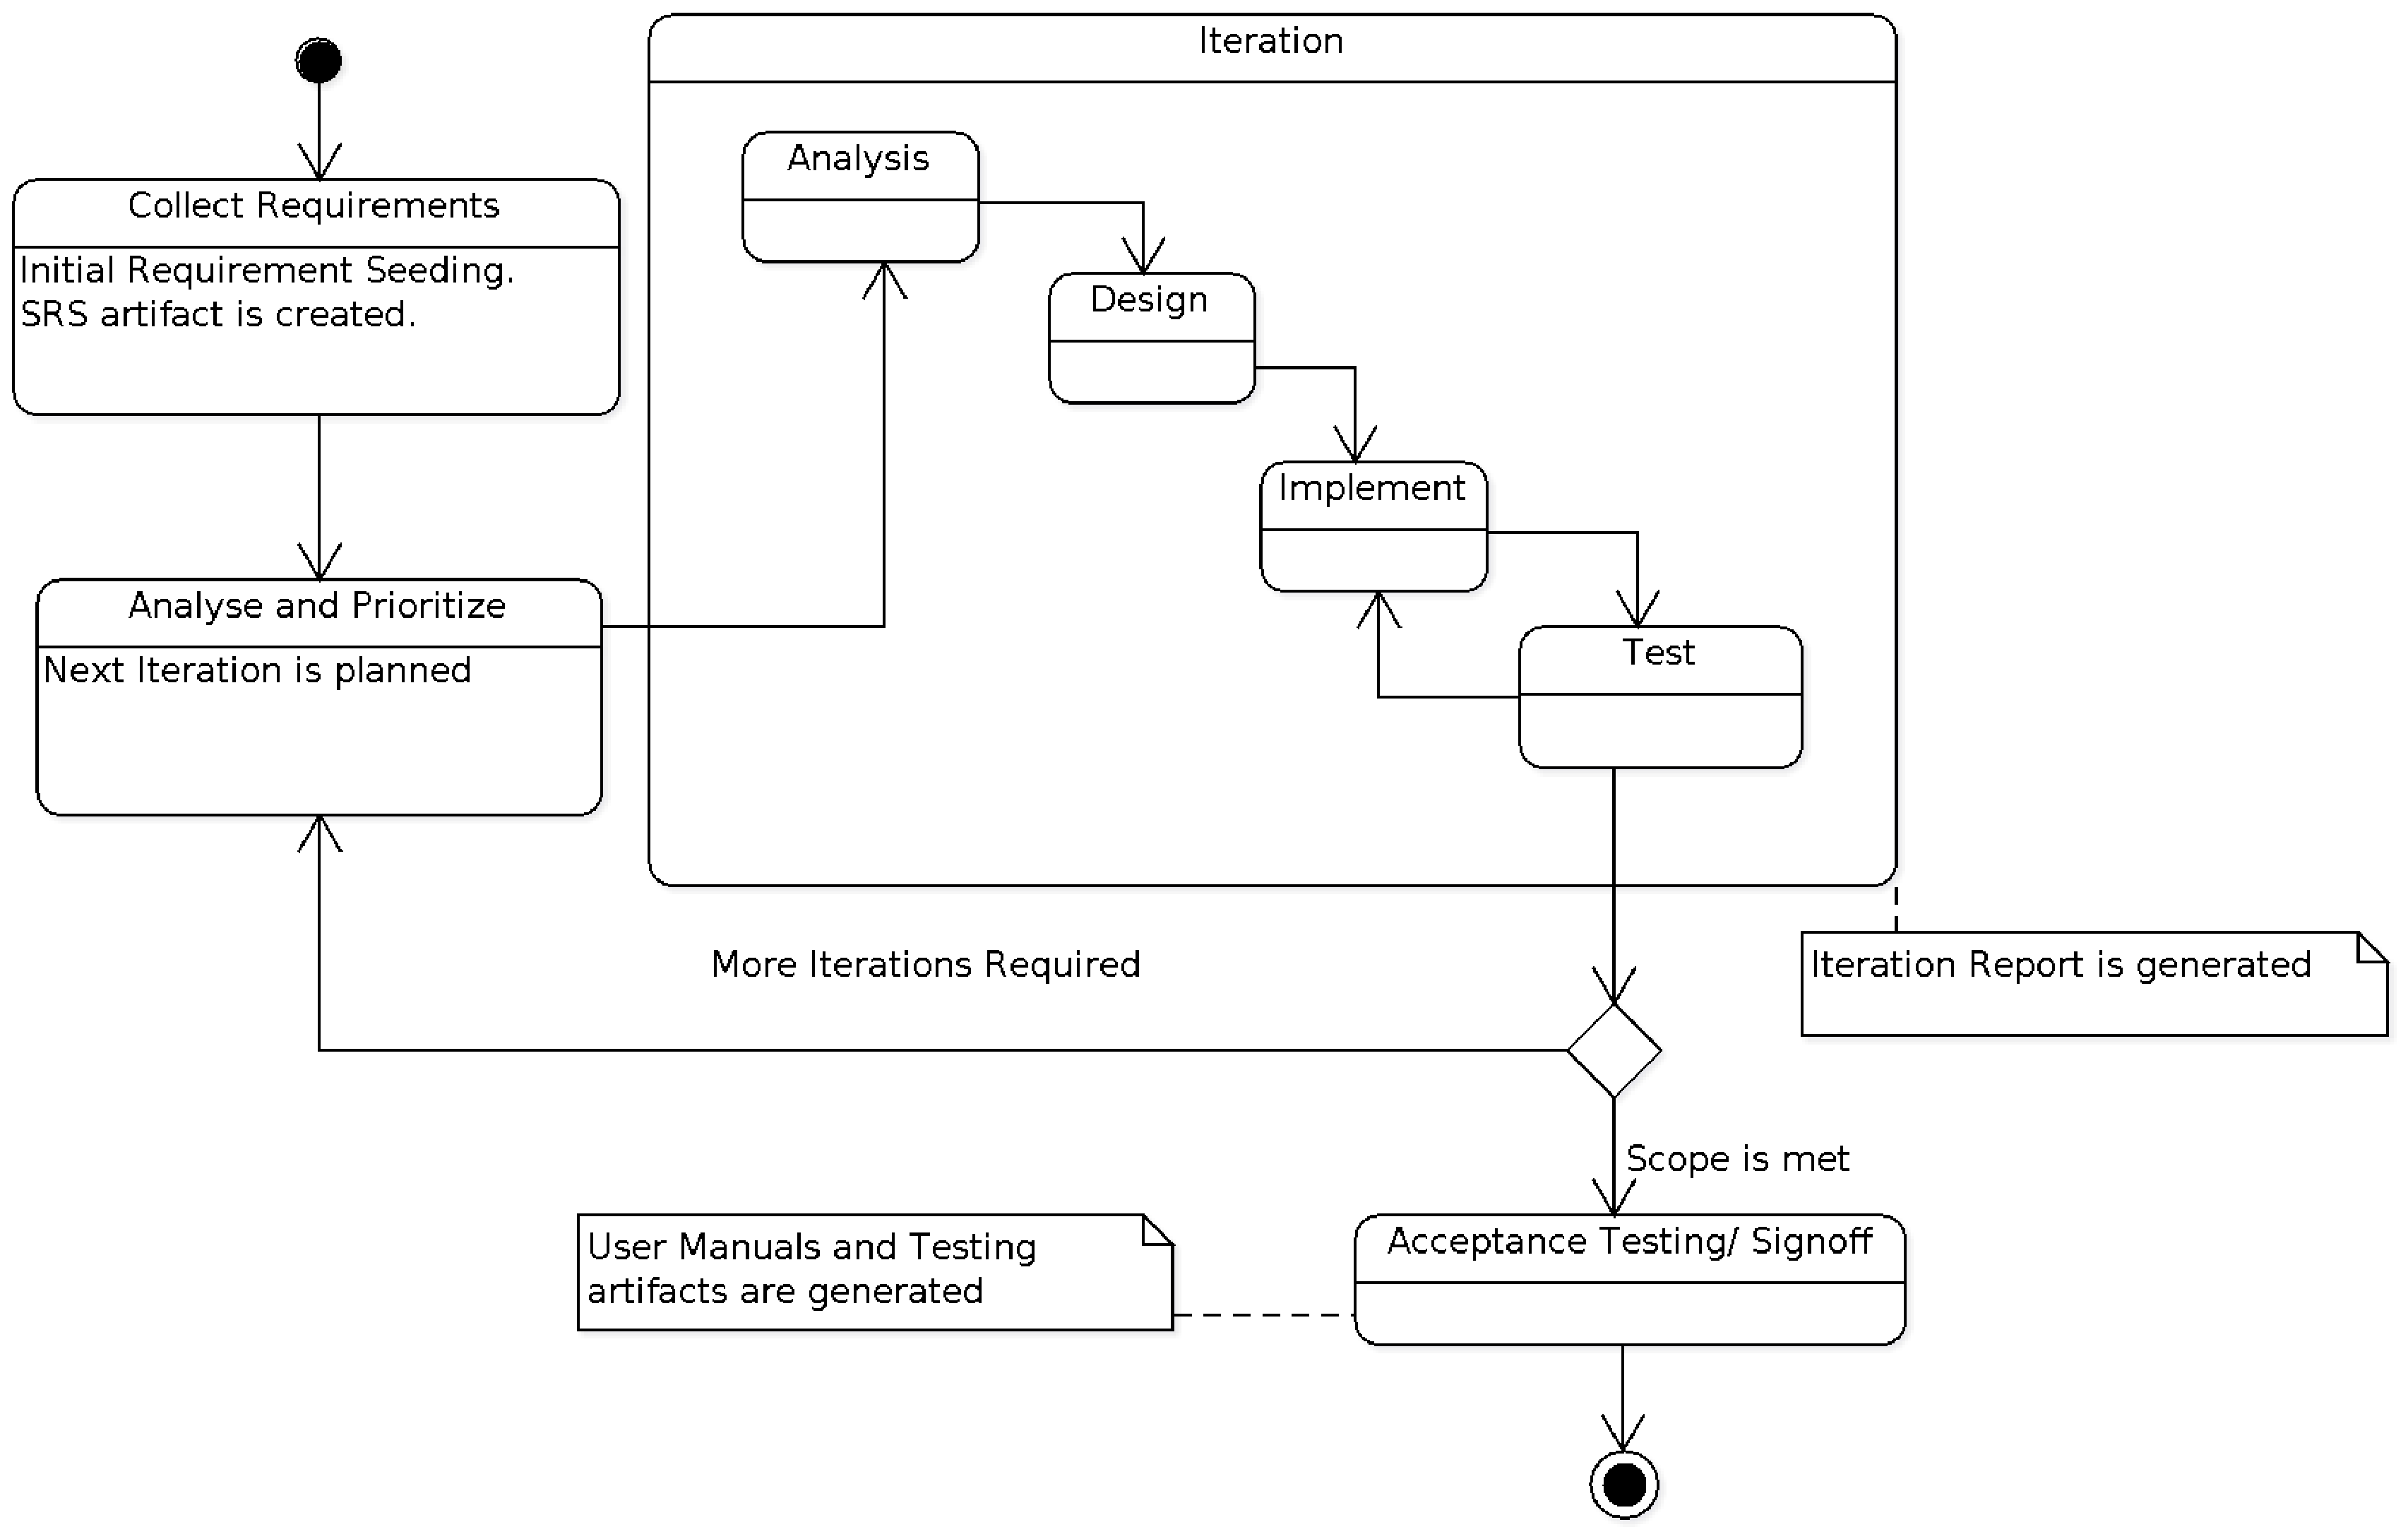
\includegraphics[width=18cm]{images/Methodology} \caption{ The proposed feature driven development } \label{fig:methods}

\end{center}
\end{figure}

\newpage

\section{Project Tasks and Resources}

\subsection{ Collaborative Tasks }

The entire project will be done as a team and several components will require collaborative work between both of us:

\begin{itemize}
\item Graphical User Interface
\item Database  Design
\item Process Workflow Design
\item Systems Analysis
\item Implementation and Testing
\item Project documentation
\end{itemize}

\subsection{ Software Tasks: Kartik Thakore }

\subsubsection{Reporting Software}

Reporting Software will be used to calculate and generate data reports as needed. Statistical Software (R Language) will be explored as an alternative.

\subsubsection{Rule Engine and Feedback Gathering System}

The system will need to follow business rules and send triggers to gather feedbacks. This system will be built on existing technology such as: Email, SMS etc. 

\subsubsection{Core Framework and Interface}

A core framework will be used to talk to databases and provide a graphical user interface to the user. Moreover several interfaces will be required to mesh with Radio Frequency Identification (RFID) and E-Signature technology. 

\subsection{ Electrical Tasks: Parth Champaneri }

\subsubsection{Network Design and Encryption:}

We will be using an iterative process to determine the most efficient design topology so that the new network meets the need for the end-users. The primary objective of this exercise to optimize the prototype network and have encryption at Application layer, Database level security and transport level security. Techniques will be implemented to minimize failures and increase protection at the server level. 

\subsubsection{Smart Access Applications:} Smart access applications will be used to enhance the experience of the end user and provide useful data for processing. Some of the applications, which will be explored, are:

RFID applications will be explored to enhance and automate the system. Some of the identified uses are implementing an attendance management device, which will record Seminar attendance for graduate students. Furthermore, it can also be used for asset management.

\subsubsection{E-Signature Pad:} The possibility of integrating a signature pad option will be explored for recording signatures after the advisory committee meeting or other processes where signatures need to be captured. This will, in turn eliminate the use of paper and we will be able to align the system to eco-sustainability initiatives supported by UWO. All the data will be stored on the server, which can be utilized for planning and analysis at a later stage.

Smart Phone Applications have revolutionized the way users interact with technology. In order to exploit the power of mobile applications, we will explore the development of a smartphone application that students can access to manage their information as well as administrative personnel. Furthermore, UPC scan codes can be implemented to facilitate student management at the seminars and advisory committees.

\subsection{Part Lists} 

\subsubsection{ Hardware Components }
\begin{itemize}
\item{Application / Database Server}
\item{RFID tag reader}
\item{E-signature pad prototype}
\end{itemize}

\subsubsection{ Software Components }
\begin{itemize}
\item{Software Licensing Costs }
\item{SmartPhone Application Development Suite (As per manufacturers requirements)}
\end{itemize}

\section{Deliverables}
\begin{itemize}
 \item{ Requirements Documentation }
 \item{ Iteration Reports (Periodic Status Reports) }
 \item{ Midterm Report}
 \item{ Final Product and Report }
\end{itemize}
\section{Project Plan}
As mentioned before, we will be using Agile project management technique to deliver the solution. As part of the methodology and as we will be delivering five iterations before a final roll-out of the prototype in March. The key advantages of this methodology are:
\begin{itemize}
\item Deliver work fast
\item Ensures that the focus always remains from the end-users perspective.

\item Very tight learning feedback loop allows for quick discovery of optimal solutions
\item Each iteration will continue for a duration of three weeks following a one week period to obtain feedback from the stakeholders and the end-users.
\end{itemize}
\newpage
\thispagestyle{empty}


 \begin{landscape}


\subsection{Gantt Chart} 
  \scalebox{0.8}{
  \begin{gantt}[xunitlength=0.65cm,fontsize=\small,titlefontsize=\small,drawledgerline=true]{16}{32}
    \begin{ganttitle}
      \titleelement{2010}{16}
      \titleelement{2011}{16}
    \end{ganttitle}
    \begin{ganttitle}
      \titleelement{Sept}{4}
      \titleelement{Oct}{4}
      \titleelement{Nov}{4}
      \titleelement{Dec}{4}
      \titleelement{Jan}{4}
      \titleelement{Feb}{4}
      \titleelement{Mar}{4}
      \titleelement{Apr}{4}
    \end{ganttitle}
    \begin{ganttitle}
      \numtitle{1}{1}{4}{1}
      \numtitle{1}{1}{4}{1}
      \numtitle{1}{1}{4}{1}
      \numtitle{1}{1}{4}{1}
      \numtitle{1}{1}{4}{1}
      \numtitle{1}{1}{4}{1}
      \numtitle{1}{1}{4}{1}
      \numtitle{1}{1}{4}{1}
    \end{ganttitle}
    \ganttbar{Problem Definition}{1}{3}
    \ganttbar{Requirements Engineering}{4}{2}
    \ganttcon{4}{3}{4}{4}
    \ganttbar{Iteration 1}{6}{3}
    \ganttcon{6}{4}{6}{5}
    \ganttbar{Iteration 1: Feedback }{9}{1}
    \ganttcon{9}{5}{9}{6}
    \ganttcon{9}{5}{9}{7}
    \ganttbar{Iteration 2}{9}{3}
    \ganttbar{Iteration 2: Feedback }{12}{1}
    \ganttcon{12}{7}{12}{8}
    \ganttcon{12}{7}{12}{9}
    \ganttbar{Iteration 3}{12}{3}
    \ganttbar{Iteration 3: Feedback }{16}{1}
    \ganttcon{15}{9}{16}{10}
    \ganttcon{15}{9}{16}{11}
    \ganttbar{Iteration 4}{16}{3}
    \ganttbar{Iteration 4: Feedback }{19}{1}
    \ganttcon{19}{11}{19}{12}
    \ganttcon{19}{11}{19}{13}
    \ganttbar{Iteration 5}{19}{3}
    \ganttcon{22}{13}{22}{14}
    \ganttbar{Acceptance Testing}{22}{2}
    \ganttcon{24}{14}{24}{15}
    \ganttbar{Project Documentation}{24}{4}  
  \end{gantt}
  }
  \end{landscape}

\newpage

\section{Advisor}
\begin{description}
\item Hanif Ladak Ph.D., P.Eng.
\item Associate Professor
\item hladak@uwo.ca 519-661-2111 x86551 
\item MSB 403
\item Signature: 
\item Date:
\item Comments:
\end{description}
\section{Grade}
\begin{description}
\item Mark of the Course Coordinator (ECE 4416): pass/fail
\item Date:
\end{description}

\newpage
\bibliography{ref}


\end{document}

